% Build (twice): pdflatex -jobname=Epiplexity_with_lightweight_learning_algorithms epiplexity_project.tex
\documentclass[aspectratio=43]{beamer}
\usetheme{default}
\usefonttheme{professionalfonts}
\setbeamersize{text margin left=7mm,text margin right=7mm}
\setbeamertemplate{navigation symbols}{}
\setbeamertemplate{footline}[frame number]
\setbeamertemplate{itemize item}{--}
\setbeamertemplate{itemize subitem}{--}
\usepackage[T1]{fontenc}
\usepackage{lmodern}
\usepackage{amsmath,amssymb,mathtools,booktabs}
\usepackage{microtype}
\usepackage{natbib}
\renewcommand{\bibsection}{}
\definecolor{myblue}{RGB}{25,75,130}
\setbeamercolor{structure}{fg=myblue}
\setbeamercolor{frametitle}{fg=myblue}
\setbeamerfont{frametitle}{size=\large,series=\bfseries}
\setbeamerfont{normal text}{size=\normalsize}
\newcommand{\KL}{\mathrm{KL}}
\newcommand{\MDL}{\mathrm{MDL}}
\newcommand{\E}{\mathbb{E}}
\title{Epiplexity with lightweight learning algorithms}
\subtitle{Experimental design for MLP, CNN and DiT setups}
\author{}
\date{September 2026}
\begin{document}
% ------------------------------------------------------------
\begin{frame}
\titlepage
\end{frame}
% ------------------------------------------------------------
\begin{frame}{Bounded observers}
Shannon entropy and Kolmogorov complexity place no limit on the computation of the observer. Epiplexity measures information relative to a time bound \citep[Def.~7--8]{finzi2026}.
\begin{definition}[$T$-time probabilistic model]
Fix a prefix-free universal Turing machine $\mathcal U$ and a time bound $T:\mathbb N\to\mathbb N$. A program $P$ is a \emph{$T$-time probabilistic model} over $\{0,1\}^n$ if, within $T(n)$ steps of $\mathcal U$, it
\begin{itemize}
\item outputs the probability $P(x)$ of any $x\in\{0,1\}^n$;
\item outputs a sample $x\sim P$ from a string of random bits.
\end{itemize}
$\mathcal P_T$ is the set of such programs; $|P|$ is the length of $P$ in bits.
\end{definition}
Logarithms are base 2.
\end{frame}
% ------------------------------------------------------------
\begin{frame}{Epiplexity and time-bounded entropy}
\begin{definition}
For a random variable $X$ on $\{0,1\}^n$, let
\[
P^* = \arg\min_{P\in\mathcal P_T}\bigl\{|P| + \E[-\log P(X)]\bigr\},
\]
with ties broken by the shortest program. Then
\begin{align*}
S_T(X) &:= |P^*| && \text{epiplexity: structure,}\\
H_T(X) &:= \E[-\log P^*(X)] && \text{time-bounded entropy: randomness,}\\
\MDL_T(X) &:= S_T(X) + H_T(X) && \text{total description length.}
\end{align*}
\end{definition}
\begin{itemize}
\item Uniform random bits: $S_T=O(1)$ and $H_T\ge n-O(1)$.
\item $S_T$ depends on $T$ and on $\mathcal P_T$; it need not grow with $T$.
\end{itemize}
\end{frame}
% ------------------------------------------------------------
\begin{frame}{Random and structural information}
\centering
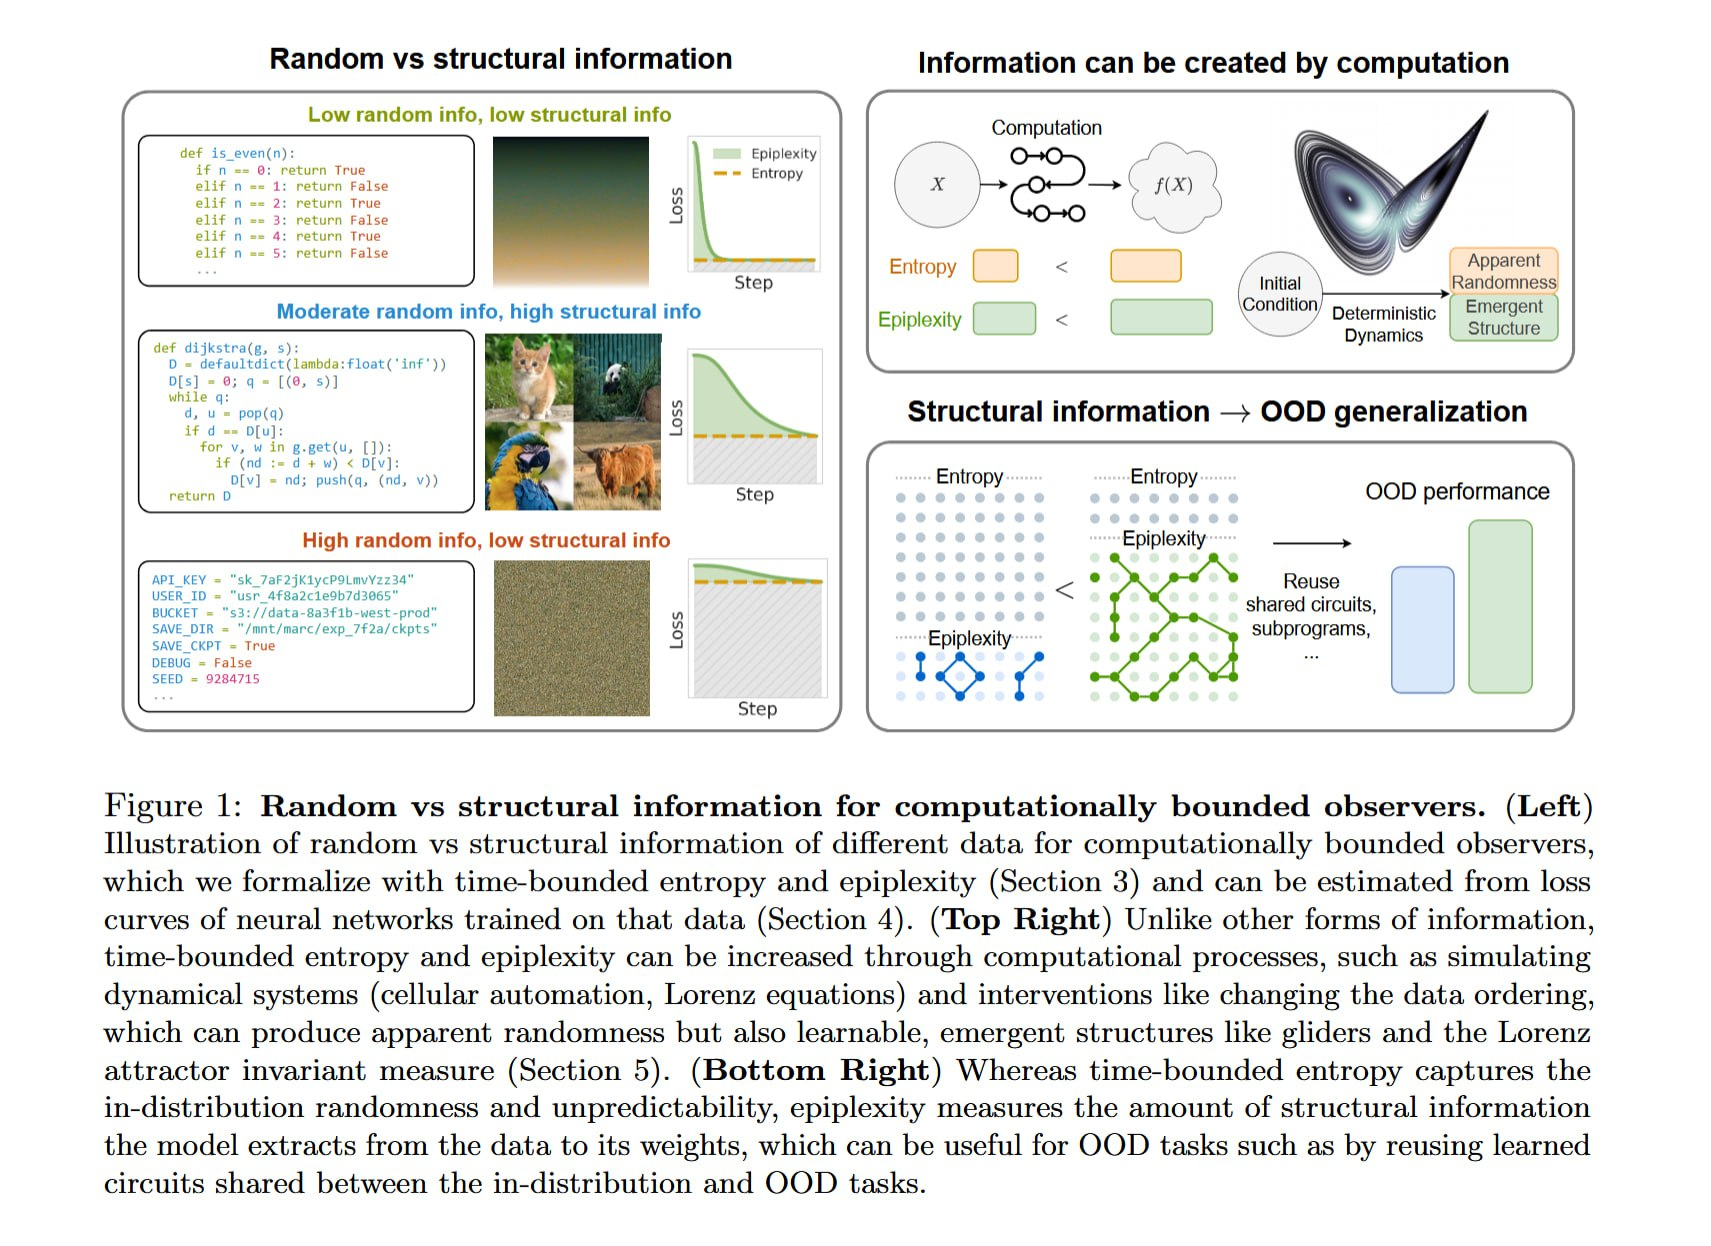
\includegraphics[width=0.9\linewidth,trim=56 267 65 16,clip]{epiplexity.jpeg}

\medskip
\raggedright\footnotesize
\textbf{Left:} a network trained on three kinds of data. The final loss approximates $H_T$ (dashed); the area above it approximates $S_T$ (green).\\
\textbf{Right:} computation can create both kinds of information; learned structure transfers out of distribution (OOD).\\
Source: Fig.~1 of \citet{finzi2026}.
\end{frame}
% ------------------------------------------------------------
\begin{frame}{From the definition to a measurement}
A \emph{setup} $a$ fixes an architecture, an optimiser, a training schedule and, for a diffusion transformer (DiT), a sampler.
\begin{itemize}
\item Compute is in FLOPs. A network with $N$ parameters, trained on $D$ examples and evaluated on the $D_X$ examples of $X$, needs $6ND+2ND_X\le T$.
\item $\mathcal P^a_T$ is the set of models that setup $a$ reaches within $T$.
\item The code length $K(P)$ of a trained model $P$ replaces $|P|$.
\end{itemize}
\medskip
The measured epiplexity is $S^a_T(X) := K(\hat P)$, where
\[
\hat P = \arg\min_{P\in\mathcal P^a_T}\bigl\{K(P) + \E[-\log P(X)]\bigr\}.
\]
We sweep $N$ and $D$. Each checkpoint gives the point $(\text{FLOPs},\ K + D_X\cdot\text{held-out loss})$; $S^a_T$ is the model part on the lower convex hull at $T$ \citep{finzi2026}.
\end{frame}
% ------------------------------------------------------------
\begin{frame}{Estimators I: prequential code and EDL}
A training run sees examples $z_0,\dots,z_{M-1}$, sampled i.i.d. Model $P_i$ is trained on $z_0,\dots,z_{i-1}$; its loss is $\ell_i(z)=-\log P_i(z)$.

\medskip
\textbf{Prequential code} \citep{finzi2026}: send $z_i$ in $\ell_i(z_i)$ bits, then train on it. The model part is the area of the loss curve above the final loss:
\[
K_{\mathrm{preq}} \approx \sum_{i<M}\bigl[\ell_i(z_i)-\ell_M(z_i)\bigr].
\]
\textbf{Excess description length} \citep{donoway2026}: the floor is the population loss $L(P)=\E_z[-\log P(z)]$ of the model $P_{\mathrm{fin}}$ at the end of training with compute $T$:
\[
\mathrm{EDL}_T = \E\sum_{i<M}\ell_i(z_i) - M\,L(P_{\mathrm{fin}}).
\]
The expectation is over the sample and its order. EDL is defined for one fixed training algorithm.
\end{frame}
% ------------------------------------------------------------
\begin{frame}{Estimator II: requential code}
Requential coding transmits a student model \citep{qiu2026}.
\begin{itemize}
\item A teacher $P^{\mathrm t}_i$ trains on real data. A student $P^{\mathrm s}_i$ trains only on samples of the teacher.
\item Encoder and decoder share the student initialisation, update rule and random seed.
\item Relative entropy coding sends one sample of $P^{\mathrm t}_i$ to a decoder that knows $P^{\mathrm s}_i$ in about $\KL_i=\KL(P^{\mathrm t}_i\,\|\,P^{\mathrm s}_i)$ bits (Kullback--Leibler divergence).
\end{itemize}
Over student steps $i$ the code length is
\[
K_{\mathrm{req}} \le \sum_i\bigl[\KL_i + 2\log(1+\KL_i) + \kappa\bigr],\qquad \kappa<5.21.
\]
Both papers report $\sum_i\KL_i$. The code contains only the disagreement of teacher and student; the entropy of the data does not enter.
\end{frame}
% ------------------------------------------------------------
\begin{frame}{What we test: the estimators, not the architectures}
The measured value depends on the data $X$, the bound $T$ and the setup
\[
a \in \{\text{MLP},\ \text{CNN},\ \text{DiT}+\text{sampler}\}.
\]
Two sources of change have to be told apart:
\begin{itemize}
\item \emph{manipulations} inside a setup: example order, input permutation, sampler, bound $T$;
\item the \emph{observer family}: hypothesis class and inductive bias.
\end{itemize}
The setup dependence is
\[
\Delta_{ab}(X,T) = S^a_T(X) - S^b_T(X).
\]
\textbf{Goal:} which part of $S^a_T(X)$ comes from $X$, which from $a$.
\end{frame}
% ------------------------------------------------------------
\begin{frame}{Benchmark: elementary cellular automata (ECA)}
\begin{itemize}
\item A row of $n$ cells takes values in $\{0,1\}$. A rule $r\in\{0,\dots,255\}$ sets each cell from itself and its two neighbours; $F_r$ updates all cells at once.
\item Task $d=(r,t)$: the input $x$ is uniform on $\{0,1\}^n$; the label is $y=F_r^t(x)$.
\item The codes cover labels only. Every estimate is then a conditional epiplexity $S_T(Y\mid X)$: the definition with $-\log P(Y\mid X)$ in place of $-\log P(X)$.
\end{itemize}

\medskip
\citet{finzi2026} report, for transformers on 64 cells and $t=48$:
\begin{center}
\begin{tabular}{lccc}
\toprule
Rule & 54 & 15 & 30 \\
\midrule
$S_T$, bits & $\approx5\times10^6$ & $\approx2\times10^5$ & $\approx0$ \\
\bottomrule
\end{tabular}
\end{center}
Rule 30 looks random to a bounded observer: its information is almost all $H_T$.
\end{frame}
% ------------------------------------------------------------
\begin{frame}{Setups and manipulations}
\begin{center}
\small
\setlength{\tabcolsep}{4pt}
\renewcommand{\arraystretch}{1.12}
\begin{tabular}{lccc}
\toprule
& MLP & CNN & DiT \\
\midrule
Parameters $N$ & $10^3$--$10^6$ & $10^3$--$10^6$ & small $\rightarrow$ medium \\
Prior & weakest & locality & generative, iterative \\
Optimiser & SGD / Adam(W) & SGD / Adam(W) & Adam(W) \\
Manipulation & example order & input permutation & sampler, \#steps \\
\bottomrule
\end{tabular}
\end{center}
\begin{itemize}
\item \emph{Example order:} the order of $z_0,\dots,z_{M-1}$. An MLP has no spatial prior.
\item \emph{Input permutation:} one fixed permutation of cells or pixels. Labels are unchanged; locality is removed.
\item \emph{Sampler:} the denoising schedule of the DiT; \#steps is the number of network evaluations per sample.
\end{itemize}
Within one comparison the task and $T$ are fixed.
\end{frame}
% ------------------------------------------------------------
\begin{frame}{Validation}
For each task $d$, setup $a$, bound $T$ and seed $s$ we compute $S_{\mathrm{preq}}$ and $S_{\mathrm{req}}$ (the value $S^a_T$ with $K=K_{\mathrm{preq}}$ or $K_{\mathrm{req}}$) and $\mathrm{EDL}_T$.
\begin{itemize}
\item \textbf{Agreement:} Spearman $\rho$ and Kendall $\tau$ between the task orderings of two estimators, within and across setups.
\item \textbf{Setup dependence:} $\Delta_{ab}$ per task, averaged over seeds. A large $\Delta$ with a stable task order means the estimate partly measures the setup.
\item \textbf{Seed variance:} the standard deviation over $s$, compared with the spread across setups.
\item \textbf{Baselines:} final test loss, sample efficiency.
\end{itemize}

\medskip
\textbf{Deliverable:} a map of where each estimator is setup-invariant.
\end{frame}
% ------------------------------------------------------------
\begin{frame}[t]{Literature}
\small
\begin{thebibliography}{99}
\bibitem[Finzi et al.(2026)]{finzi2026}
M.~Finzi, S.~Qiu, Y.~Jiang, P.~Izmailov, J.~Zico Kolter, A.~G.~Wilson.
\newblock \emph{From Entropy to Epiplexity: Rethinking Information for Computationally Bounded Intelligence}.
\newblock arXiv:2601.03220, 2026.
\bibitem[Qiu et al.(2026)]{qiu2026}
S.~Qiu, M.~Finzi, Y.~Zheng, K.~Zhang, A.~G.~Wilson.
\newblock \emph{Requential Coding: Pushing the Limits of Model Compression with Self-Generated Training Data}.
\newblock arXiv:2607.11883, 2026.
\bibitem[Donoway et al.(2026)]{donoway2026}
E.~Donoway, H.~Joren, F.~Roger, J.~Leike.
\newblock \emph{Excess Description Length of Learning Generalizable Predictors}.
\newblock arXiv:2601.04728, 2026.
\end{thebibliography}
\end{frame}
\end{document}
